\documentclass[11pt]{article}
\renewcommand{\baselinestretch}{1.20} 
\usepackage[utf8]{inputenc}
\usepackage[english]{babel}
\usepackage{graphicx}
\usepackage{wrapfig}
\usepackage{subcaption}
\usepackage{geometry}
\usepackage{xcolor}
\usepackage{float}
\usepackage{mdframed}
\usepackage{fancyhdr}
\usepackage{lastpage}
\usepackage{booktabs}% http://ctan.org/pkg/booktabs
\newcommand{\tabitem}{~~\llap{\textbullet}~~}
\geometry{a4paper, total={170mm,237mm}, left=20mm, top=20mm}
\setlength{\abovecaptionskip}{15pt plus 3pt minus 2pt}

\pagestyle{fancy}
\fancyhf{}
\rfoot{Side \thepage \hspace{1pt} / \pageref{LastPage}}
\begin{document}
    
    % Title page
    \begin{titlepage}
    \centering
	
\includegraphics[width=0.35\textwidth]{Projectdoc/Assets/Illustrationer/aau_logo_en.pdf}\par\vspace{1cm}
	{\scshape\Large Struktureret System Udvikling\par}
	\vspace{0.2cm}
	{\huge\bfseries Workshop 1\par}
	\vspace{0.2cm}
	{\scshape\Large ITC - B125\par}
	\vspace{2cm}
	{\Large\itshape 
    	Mikkel Steen Hansen\\
        Martin Boe\\
        Benjamin Bach Jensen\\
        Daniel Vestergaard Jensen\\
    \par}
	\vfill
	\vfill
\end{titlepage}
    
    % Table of contents
    \renewcommand{\baselinestretch}{0.8}
    \tableofcontents
    \renewcommand{\baselinestretch}{1.20}
    \newpage
    
    \section{Beskrivelse}
    \textbf{Mini projekt: Vejr station}\\
    Dagens workshop omhandler at videre udvikle på sidste workshops vejr station for anvendelse i et parcel hus. \\
    Tanken er at forskellige sensorer registrerer en eller flere informationer der skal til for at beskrive vejret. Disse data samles op via en enhed der kan videregive information til en app på brugerens smartphone eller computer, evt. krydret med en præcis vejrudsigt i den kommende time ved at udnytte services fra DMI
    eller anden vejr tjeneste.
    
    % Class diagram description
    \noindent
I denne workshop er fokus lidt ændret fra tidligere Workshop. Dette er grundet at tidligere Workshop hovedsageligt havde fokus på projektets login funktionalitet og de dertilhørende usecases. Til denne workshop har gruppen dog vedtaget at det mere oplagt at videre specificere projektets andre dele, her tale om interaktion og implementering.

\begin{figure}[H]
    \centering
    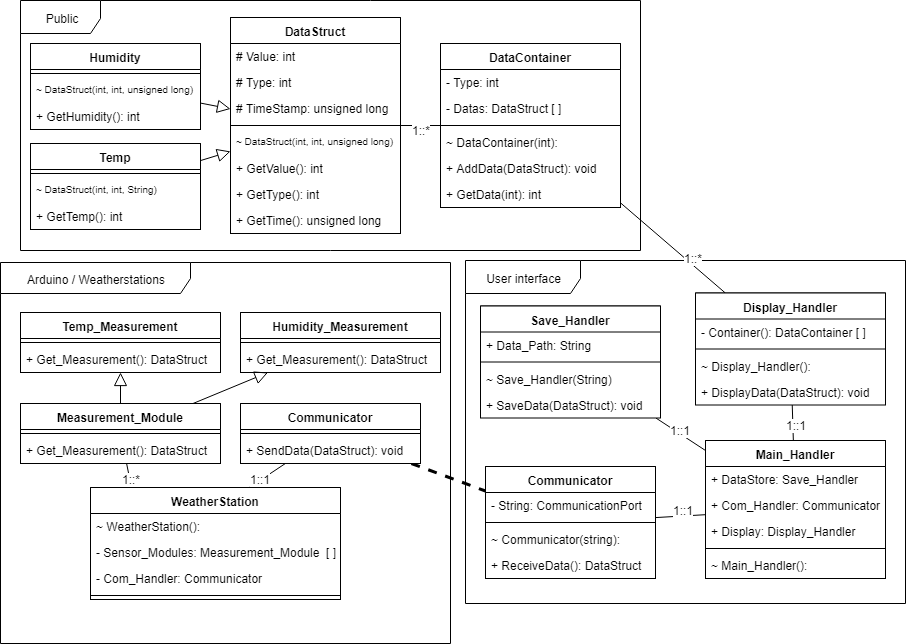
\includegraphics[width=1\textwidth, angle =0]{Struktureret_System_Udvikling/Workshop_2/Assets/Workshop2_ClassDiagram.png}
    \caption{Interaction Class Diagram}
    \label{fig:my_label}
\end{figure}

\noindent
Som ses på overstående klassediagram kan implementationen af Vejrstationen og dens kommunikation, indeles i tre generelle hovedpunkter til den videre implementation.\\
1. kaldet Public:
Der generelt beskriver funktionaliteter anvendt af både Vejrstationens egen implementation, men også af eventuelle Userinterface.
I denne kan f.eks. ses en beskrivelse af en Data Container "Data\_Struct", lavet til at kunne håndtere alle former for data sendt i en enten intern eller ekstern kommunikations forbindelse.\\
2. kaldet Arduino / Weatherstations:
Denne beskriver generelt funktionaliteten implementeret i Vejrstationen alene, dog her både til at anskaffe data, fra hvert enkelt sensor modul, men også til at håndtere, samt videresende samme data til eventuelle udestående Userinterface.\\
3. kaldet Userinterface:
Som generelt beskriver den nødvendige implementation til håndtering og visning af data'en, her modtaget fra en Verstation, og den videre mulige interaktion mellem platformen og brugeren.

Til transformation af Data mellem Verstation og Userinterface, har gruppen valgt at opbygge følgende API:

\end{document}